\subsubsection{Data integrity, security and encryption} \label{section:analysisencryption}
It is very important that the user data is securely stored and is only viewable and modifiable by the actors, that are granted the permission. User data, which ends up being transparent by default when storing it on a blockchain, needs to be encrypted for privacy reasons, by using a robust cryptographic system. Communication channels between the front-end and the back-end (or a blockchain in case of the decentralized implementation) needs to be secure to prevent the intruders from intercepting the data, or perform a "man-in-the-middle attack". Apart from the "man-in-the-middle" attack, there are numerous other ways to hack a system, or tamper with its data. It is important to be aware of potential security risks, regarding each model of implementation. From the standpoint of data integrity and security, nothing comes close to being as good as a public blockchain.

\paragraph{Data persistence and integrity}
All of the data, that is added onto a public blockchain is immutable and cannot be removed. This is possible due to cryptographic bonds between the blocks in such a way, that a new block is indirectly connected to each of the previous blocks (i.e. new block's hash is dependent on the hash of the previous block, whose hash is dependent on its previous block's hash, etc.). Every block's hash is also dependent on the block's contents, which is defined by the merkle root of all the transactions, which are included in that particular block \citep{merkle}. Thus, even an insignificant change of a given block's contents affects all of the following blocks. This hostile change would easily be detected by the consensus protocol and discarded.

All of these features contribute towards blockchain being a near 100\% persistent data structure. The benefit of that data persistence is that the user can be sure about all of the information in a blockchain being verified and unchanged. This becomes rather important, when dealing with a network that supports digital assets, as this enables a trusted prevention of double spending problem and a trusted mechanism for the trace of payments. There is near to no risk regarding loss of data, as it is stored across multiple nodes and is cryptographically secured. The combination of blockchain's data integrity and absence of a third party results in a relatively high degree of trust.

When using a system with a database, the users may never be completely sure whether the data has not been tampered with by an intruder or an insider, which is related to the third party that runs and maintains the servers. This is the case because the data is typically not available for public audits and there, theoretically, is nothing that prevents the central organization, that is in control of the databases, from changing the values in the database fields. There are no cryptographic bonds between the entries in the tables, thus reducing the data persistence quality attribute, compared to blockchain based systems.

\paragraph{DDoS attacks}
Distributed denial-of-service attack, or \textit{\glspl{DDoS}}, is a cyber-attack, in which the attacker seeks to make a machine or network resource unavailable to its intended users by temporarily or indefinitely disrupting services of one or multiple hosts. Denial of service is typically accomplished by flooding the targeted machine or resource with requests in an attempt to overload systems and prevent some or all legitimate requests from being fulfilled \citep{ddos}.

DDoS attacks are experienced by the data centers in client-server oriented services on daily basis. Even though, the DDoS attacks are becoming more and more common and advanced, the protection systems are keeping up at a good pace. There are numerous data center protection solutions out there. Most protection services are using the approach of migrating data, during DDoS attacks, like the A10 Networks Thunder TPS Solution among others \citep{a10networks}. Services like Cloudfare are using advanced traffic filtering algorithms, along with data migration to achieve complete DDoS protection, as advertised on their website \citep{cloudfare}. It is very important to use proper DDoS protection for centralized applications in order to minimize risks of downtime.

When dealing with Ethereum, there are built in mechanisms to directly and indirectly provide DDoS protection. A recepie for a successful DDoS attack is to create congenstion rate greater than, or close to the network's maximum throughput. Ethereum's throughput is defined by block gas limit and target block time, as described in \ref{section:scalability}. During a DDoS attack the gas limit of the new blocks would quickly be reached, thus increasing the pool of pending transactions that are awaiting confirmation. As the frequency of new block addition is kept the same at approximately 15 seconds, an attacker could theoretically send a lot of transactions, fill every block with them and quickly overflow the network. Technically, this would be rather easy to achieve. However, each and every transaction consumes gas, which has to be paid for (see Section \ref{section:economics}). Thus, the attacker would have to pay for each individual DDoS transaction. It is possible to pay 0 Gwei for gas, however, these transactions would not be prioritized by miners, thus making it impossible to create a DDoS attack with them. In order to occupy nearly all of the throughput, the attacker needs to assign high gas prices, which would result in the hostile DDoS transactions being prioritized over regular transactions, that have lower gas limit. The cost of performing a DDoS attack is described in following equation:

\begin{align}
C_{\mathrm{att}} &= Q_{\mathrm{gas}}  \cdot C_{\mathrm{Gwei}} \cdot T_{\mathrm{net}} \cdot P_{\mathrm{att}} = Q_{\mathrm{gas}}  \cdot C_{\mathrm{Gwei}} \cdot \frac{L_b}{t_b} \cdot P_{\mathrm{att}}
\end{align}

Here, $T_{\mathrm{net}}$ is Ethereum's network throughput, defined by Equation (\ref{eq:eththroughput}). The block time $t_b$ is 15 seconds, or 1/240 hours. Gas price $C_{\mathrm{gas}}$ is the gas price chosen by the attacker, $C_{\mathrm{Gwei}}$ is current price of one Gwei ($10^{-9}$ ETH) in terms of fiat currency. Gas block limit $L_{b}$ is equal to approximately $8 \cdot 10^6$ gas at the time of writing. Percentage of hostile transactions $P_{\mathrm{att}}$ is a measure of total desired hostile congestion rate of the attack (0.8 means that 80\% of the transactions in each block are hostile), assuming that nearly all other transactions have lower gas limit than the corresponding $C_{\mathrm{gas}}$. This yields a linear function for the cost of attack $C_{\mathrm{att}}$:

\begin{align} \label{eq_1}
C_{\mathrm{att}} &\approx C_{\mathrm{gas}}  \cdot 10^{-9} \cdot C_{\mathrm{Gwei}} \cdot 8 \cdot 10^{6} \cdot 240 \cdot P_{\mathrm{att}}\\
C_{\mathrm{att}} &\approx 1.92 \cdot C_{\mathrm{gas}}  \cdot  C_{ETH} \cdot P_{\mathrm{att}}
\end{align}

\begin{figure}[H]
\centering
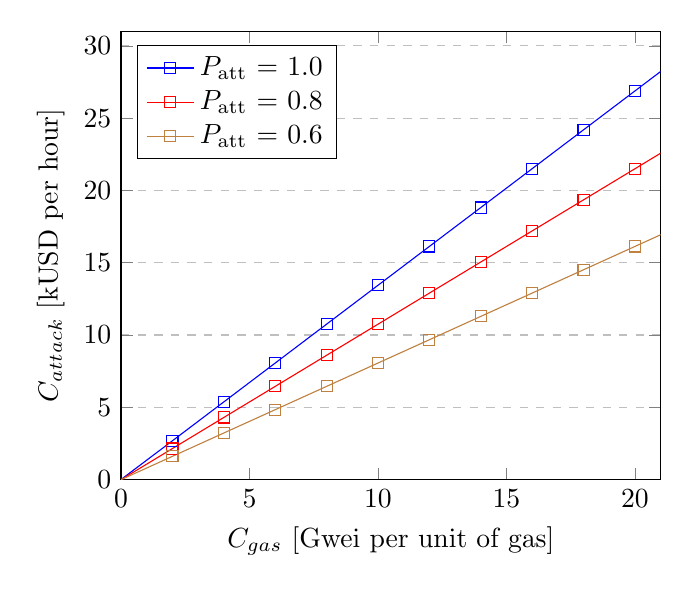
\begin{tikzpicture}
\begin{axis}[
    xlabel={$C_{gas}$ [Gwei per unit of gas]},
    ylabel={$C_{attack}$ [kUSD per hour]},
    xmin=0, xmax=21,
    ymin=0, ymax=31,
    xtick={0,5, 10, 15, 20},
    ytick={0, 5, 10, 15, 20, 25, 30},
    legend pos=north west,
    ymajorgrids=true,
    grid style=dashed,
]
 
\addplot[
    color=blue,
    mark=square,
    ]
    coordinates {
    (-2,-2.668)(2,2.688)(4,5.376)(6,8.064)(8,10.752)(10,13.440)(12,16.128)(14,18.816)(16,21.504)(18,24.192)(20,26.880)(22,29.568)
    };
    
\addplot[
    color=red,
    mark=square,
    ]
    coordinates {
    (-2,-2.150)(2,2.150)(4,4.300)(6,6.450)(8,8.600)(10,10.750)(12,12.900)(14,15.050)(16,17.200)(18,19.350)(20,21.500)(22,23.650)
    };
    
\addplot[
    color=brown,
    mark=square,
    ]
    coordinates {
    (-2,-1.612)(2,1.612)(4,3.226)(6,4.838)(8,6.451)(10,8.064)(12,9.676)(14,11.289)(16,12.902)(18,14.515)(20,16.128)(22,17.741)
    };
    \legend{$P_{\mathrm{att}}$ = 1.0, $P_{\mathrm{att}}$ = 0.8, $P_{\mathrm{att}}$ = 0.6}
 
\end{axis}
\end{tikzpicture}
\caption{Hourly cost of a theoretical DDoS attack in thousands of USD.}
\label{fig:ethddos}
\end{figure}

As can be seen in Figure \ref{fig:ethddos}, even when the attacker pays only 2 Gwei for single unit of gas and desires to establish a 60\% reduction of throughput (which would not harm the Ethereum network significantly at current state) by generating hostile transactions, it would come at a cost of approximately 2.30 ETH, or 1612 USD$^\star$ per hour. Gas price of 2 Gwei is considered to be a standard price at the time of writing. It is used in transactions for confirmations times of around few minutes, when network is moderately congested. As mentioned before, attackers would need to use a much higher gas price to block the significant part of network's throughput. A more realistic figure to look at would be gas price of around 10-15 Gwei and $P_{\mathrm{att}}$ of 0.8. An hour of such an attack would cost tens of thousands of dollars to perform. Even if the attack is performed using transactions with high gas price $N$, regular users would still be able to generate transactions and get them added to new blocks by simply using gas price of $\geq N$, which is larger then the DDoS transactions' gas price.

One more thing to consider, regarding DDoS attacks on Ethereum, is that the gas block limit is gradually increasing, as the total network hashpower grows. Recent increase from approximately $6.7 \cdot 10^6$ to around $8 \cdot 10^6$ gas happened in December 2018. Further growth of block gas limit would make theoretical DDoS attacks even more expensive, as it would lead to increased throughput of the network.

\paragraph{51\% attacks}
One of the most common potential threats to public blockchain-based systems are the \textit{\glspl{51 attack}}. The consensus principal in most blockchain based systems is indeed very much the same, as how the presidential elections in democratic countries are held, namely that the candidates need to gain the majority of votes, in order to be elected. The same principal is applied in nearly all public blockchains. In order for a new block to be added, it has to be accepted by the majority of nodes. Thus, 51\% attack refers to an attack on a blockchain by a group of miners controlling more than 50\% of the network's mining hashrate, or computing power. The possession of a total hashrate percentage of over 50\% would result in potential attackers being able to prevent new transactions from gaining confirmations, allowing them to halt payments between some or all users. They would also be able to reverse transactions that were completed while they were in control of the network, meaning they could double-spend digital assets. However, if such an attack was to take place, the attackers would still be unable to change the contents of previous blocks or generate new coins and tokens in cryptocurrency-related blockchains.

In case of Ethereum, such an attack would be possible, but highly unlikely to happen. Mining in general is such a popular activity nowadays, making Ethereum's hashrate relatively high, as shown in Figure \ref{fig:ethereumhashrate}. Therefore, the possession of more that 50\% of Ethereum's hashrate by a single person or organization is very unlikely, as it requires enormous resources. However, this enormous popularity and huge hashrate of Ethereum has resulted in solo mining being no longer viable, as the time to confirm a block by mining solo is often measured in months, or even years in case of some popular networks, depending on the size of mining operation and luck factor. This led to the introduction of, so called, \textit{\gls{pool mining}}. Its concept is that the miners join a pool, which distributes nonces to different mining subnodes (in other words, miners are cooperating between eachother to find blocks, when pool mining). Miners then get a share of total block reward from the blocks that have been found by the pool. This basically means that the mining pool is being in the possession of all the contributed hash power. This can lead to security concerns if the pool's total hashrate becomes more than a half of the total network hashrate, as it enables the pool to execute such 51\% attack.

\begin{figure}[H]
\centering
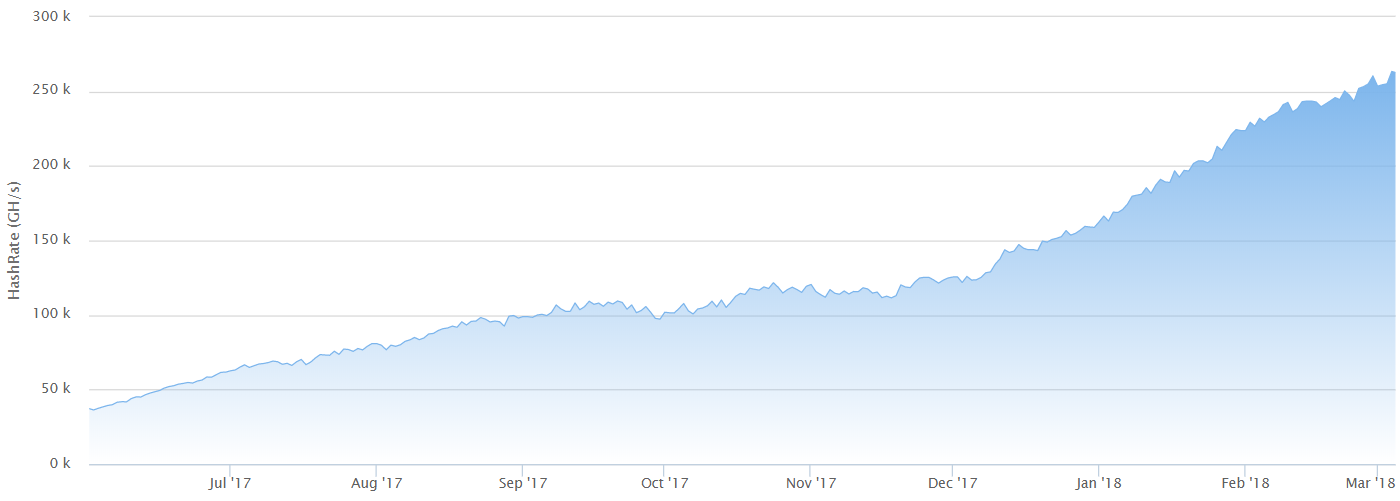
\includegraphics[scale=0.49]{images/ethereumhashrate.png}
\caption{Overall Ethereum network hashrate \textnormal{\citep{ethhashrate}}.}
\label{fig:ethereumhashrate}
\end{figure}

However, hitting 51\% network control is not a guarantee of success, it is just the point where success is likely. In fact, a node could attempt this sort of attack with much less network control, but the odds of success would be very low \citep{51perattack}. 

There is an obvious conclusion that can be drawn, regarding the 51\% attacks. Network's exposure to such attacks proportionally decreases, when the overall network hashrate increases. Smaller blockchain networks are obviously more exposed to 51\% attacks, than larger, more popular networks, that possess higher hashrates.

\paragraph{Man-in-the-middle attacks}
A \textit{\gls{man-in-the-middle attack}} is a type of cyberattack, in which a malicious actor inserts him/herself into a conversation between two parties, impersonates both parties and gains access to information that the two parties were trying to send to each other. In case of such attack, a malicious actor may try to intercept, send and receive data meant for someone else, or not meant to be sent at all, without either outside party knowing until it is too late \citep{mitm}.

Any system, that communicates via the Internet is exposed to such attacks. Thus, the communication channel between the user and the service, whether it is a blockchain or a server, has to be secure. A common technique, which is used in order to achieve that is digital signatures. Digital signatures ensure that the contents of the message, which was transmitted through the channel, were not tampered with, or changed.

\paragraph{Smart contracts and security flaws}
Ethereum is an extremely secure network. As was discussed before, it has a sufficient enough protection against 51\% attacks and DDoS attacks are extremely costly and impractical to perform. However, it is still possible to implement buggy smart contracts, that would introduce potential security flaws. The DAO hack, which was briefly mentioned in \ref{section:transparency}, happened due to that particular reason, as there was a bug in the DAO smart contract, which was discovered by the attacker and exploited. Thus, the developers need to be extremely careful, during the implementation process, in order to prevent such events from happening. A tool, which might be useful for that purpose is called Oyente. This tool can be used to test the smart contract code for bugs and security breaches \citep{oyente}.

\paragraph{Encryption in centralized systems}
There are many cryptographic solutions that can be chosen for the implementation of centralized systems. There are countless different algorithms out there, that are typically using two main cryptographic approaches: symmetric and asymmetric.

\textit{\Gls{symmetric encryption}} is the simplest kind of encryption that involves only one secret key to cipher and decipher information. Symmetrical encryption is an old and best-known technique. It uses a secret key that can either be a number, a word or a string of random letters. It is a blended with the plaintext of a message to change the content in a particular way. The sender and the recipient should know the secret key that is used to encrypt and decrypt all the messages. Blowfish, AES, RC4, DES, RC5, and RC6 are examples of symmetric encryption. The most widely used symmetric algorithm is AES-128, AES-192, and AES-256. The old and outdated DES algorithm is now used in a 3DES configuration, which basically involves execution of DES three times. The main disadvantage of the symmetric key encryption is that all parties involved have to exchange the key used to encrypt the data before they can decrypt it.

\textit{\Gls{asymmetric encryption}} is also known as public key cryptography, which is a relatively new method, compared to symmetric encryption. Asymmetric encryption uses two keys to encrypt a plaintext. It is important to note that anyone with a secret key can decrypt the message and this is why asymmetrical encryption uses two related keys to boosting security. A public key is made freely available to anyone, while private key is kept a secret. A message that is encrypted using a public key can only be decrypted using a private key, while also, a message encrypted using a private key can be decrypted using a public key. Security of the public key is not required because it is publicly available and can be passed over the Internet. Asymmetric key has a far better power in ensuring the security of information transmitted during communication. Asymmetric encryption is mostly used in day-to-day communication channels, especially over the Internet. Popular asymmetric key encryption algorithm includes RSA, DSA, Elliptic Curve (used in Ethereum and many other blockchains), PCKS and others \citep{pubvssym}.

\begin{figure}[H]
\centering
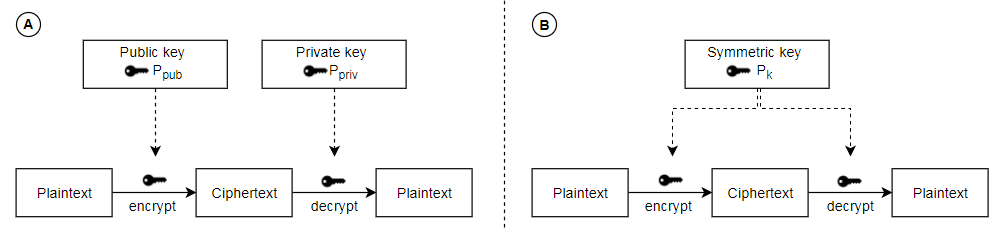
\includegraphics[scale=0.55]{images/pubpriv.png}
\caption{Public key cryptography (A) and symmetric encryption (B) illustrations.}
\label{fig:keygenerationether}
\end{figure}

Different encryption algorithms are good in different aspects and bad in other ones. For example, symmetric encryption algorithms are significantly faster than the asymmetric ones, however, they involve transmission of private keys before the communication can take place, thus introducing a risk of private key being intercepted. It is important to use encryption algorithms that are right for the task at hand.

\paragraph{Possible encryption mechanism in smart contracts}
Theoretically, the smart contracts can easily store 256-bit application-specific public keys of addresses, using data structure, called \texttt{mapping}. It maps key value pairs, where the keys could potentially correspond to users' Ethereum addresses and the values could correspond to the application-specific public keys. As mentioned in \ref{section:transparency}, Ethereum is completely transparent, thus the sensitive private information of users in the blockchain based Secure Package system would be exposed to the public, if not encrypted. 

The solution for that could be to generate individual Secure Package key pairs off-chain, store private keys securely at the user's computer and upload public keys to corresponding mappings inside of the smart contract. The reason behind generation of keys off the chain is that it prevents serious security and efficiency issues with on-chain generation.

Thus, it is theoretically possible to create encryption protocols for data transfer and storage in Ethereum. The keys would need to be 256-bit long, while still being able to provide secure encryption that can withstand hostile intrusion attacks. This can be achieved with elliptic curve cryptography in rather the same manner, as how Ethereum addresses' key pairs are generated. This is covered in greater detail in the next paragraph.

\paragraph{Key distribution and generation in Ethereum}
Public key cryptography is widely used in blockchain-based systems. Private keys are used to sign the transactions and generate public keys. As mentioned before, the Ethereum blockchain is completely transparent. This makes generation and distribution of private keys on-chain a very bad idea, as the keys can be intercepted by anyone, thus making them useless.

To solve these issues, the private key generation process for new Ethereum accounts is performed off-chain by taking any random 256-bit number and storing it safely off-chain. This 256-bit number acts as a private key. Public key is then generated from that random private key, which in its turn generates the account address. Key pairs are used for verification purposes and the address is used for indexing.

\begin{figure}[H]
\centering
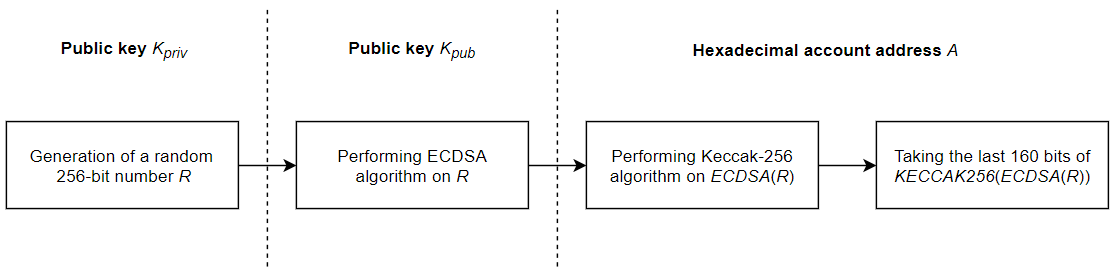
\includegraphics[scale=0.62]{images/ethaddr.png}
\caption{Generation of keys and addresses in Ethereum. Private key is stored off-chain. Generation process involves the ECDSA algorithm, along with Keccak256 hashing algorithm \textnormal{\citep{ethyellow}}.}
\label{fig:keygenerationether}
\end{figure}

Using this approach, the private key is never being sent over the blockchain. This makes it very difficult for the intruder to access the account, assuming that a properly chosen seed has been used to randomly generate the private key. The are theoretically only two ways to break such 256-bit ECDSA private key. The first and most straightforward way would be to try all of the possible key combinations, which might take billions of years with the current technology, as there are $2^{256}$ possible keys. This approach is often referred to as "brute force". The second way is to solve the Elliptic Curve Discrete Logarithm Problem (ECDLP), which the ECDSA algorithm is based on. Rough estimates of solving this problem by using raw processor power is around $38.5 \cdot 10^{20}$ years, assuming that the encryption has been done properly and that private key possesses high degree of randomness. There are other approaches to solving this problem, by exploiting mathematical properties, such as hyperelliptic curves and elliptic curves with small complex multiplication fields \citep{ecdsa}.

Ethereum's public key cryptography, which is based on ECDSA, is considered being very secure, despite using rather short key size, compared to RSA, in which key lengths of up to 4096 bits are used \citep{rsakeys}. This has to do with the complexity of underlying mathematical problem. The mathematical problem that RSA is based on is prime number factorization, which is a lot less complex than ECDLP. That is the reason for a rather short key size in ECDSA.

Nevertheless, as long as the private key file is securely stored on the user's computer, there is little to no risk of the account being broken by an intruder.
